\documentclass[10pt, conference, compsocconf]{IEEEtran}
\usepackage[nocompress]{cite}
\usepackage[font=normalsize,labelfont=sf,textfont=sf]{subfig}
\usepackage{graphicx}
\usepackage{arabtex}
\usepackage[cmex10]{amsmath}

%packages that were not copied from the IEEE template - need to check if it is valid to add them
\usepackage{amssymb}
\usepackage[linesnumbered]{algorithm2e}
\usepackage{color}

\begin{document}

\title{Ongoing Segmentation of On-line Handwritten Arabic Script}

\author{\IEEEauthorblockN{George Kour}
\IEEEauthorblockA{Faculty of Engineering\\
Tel-Aviv University\\
Tel-Aviv Jaffa, Israel\\
Email: kourgeorge@gmail.com}
\and
\IEEEauthorblockN{Raid Saabne}
\IEEEauthorblockA{Department of Computer Science\\
Tel Aviv-Yaffo Academic Collage, Israel\\
Triangle R\&D Center, Kafr Qara, Israel\\
Email: saabni@cs.bgu.ac.il}
}


%\markboth{Journal of \LaTeX\ Class Files,~Vol.~6, No.~1, January~2007}%
%{Shell \MakeLowercase{\textit{et al.}}: Bare Demo of IEEEtran.cls for Computer Society Journals}


\IEEEcompsoctitleabstractindextext{
\begin{abstract}
the cursive and unconstrained nature of the Arabic script, in both printed and handwritten forms, anneals the task of segmentation. 
While real-time performance is required in applications involving on-line handwriting recognition, most techniques for handwriting recognition wait until the entire curve is traced out before starting the analysis, inevitably causing delays in the recognition process. 
This paper proposes a novel, ongoing, recognition-based segmentation technique of the on-line Arabic script, by carrying out the most time consuming recognition process while the stroke is being scribed. 
The system has been designed and tested using the ADAB Database, and promising results were obtained.\\
\end{abstract}

\begin{IEEEkeywords}
Arabic Script Segmentation, Strokes Segmentation, On-line Text Recognition, Word Segmentation, Arabic OCR
\end{IEEEkeywords}
}
\maketitle

\section{Introduction}
Handwriting remains the most commonly used mean of communication and recording of information in the daily life; therefore, a growing interest in the handwriting character recognition field has emerged in recent years. 
Handwriting recognition can be categorized into two main fields: off-line and on-line. 
In the off-line case, a digital image containing text is fed to the computer, and then the system attempts to convert the spatial representation of the letters into digital symbols \cite{al2011online}. 
On the contrary, in on-line handwriting recognition, the process is done on a digital representation of the text written on a special digitizer, PDA, tablet or smart-phone device where sensors pick up the pen-tip movements.\\
 
Techniques for cursive text recognition can be split into two main approaches. 
The holistic approach considers the global properties of the written text and recognizes the input word shape as a whole \cite{biadsy2011segmentation, saabni2009hierarchical}. 
The analytic approach involves segmentation and classification of each part of the text \cite{abdulla2008off, sari2002off, Dinges2011}. 
The holistic approach requires the classifier to be trained over the entire dictionary. 
While this is possible for a small vocabulary of words, it is impractical for large dictionaries containing 20,000 words or more \cite{elanwar2012unconstrained}.\\

The cursiveness of the Arabic script, prima facie, requires delaying the launch of the recognition process until the completion of the word scribing. 
However, in this paper, we question the necessity of the requirement by demonstrating significant acceleration of the recognition process, which was achieved by approximating the position of the segmentation points (SPs) while the stroke is being written.\\

In Section \ref{sec:related_work}, we mention related studies done in the field of on-line Arabic recognition. 
The proposed approach is described in detail in Section \ref{sec:approach}. Experimental results and analysis is given in Section \ref{sec:results}. \\

\section{Related Work}
\label{sec:related_work}

Randa et al. \cite{elanwar2012unconstrained} proposed a two stage on-line Arabic handwritten text segmentation system based on Hidden Markov Model (HMM). 
In the first stage, SPs were nominated, and then, in a second stage, the nominated points were validated using a rules-based engine. 
The system was tested using a self-collected database named OHASD.\\

Digness et al. \cite{Dinges2011} used a segmentation-based recognition approach based on dividing the word into smaller pieces, which were afterwards segmented into candidate letters, and then classified into letter classes using statistical and structural features. 
The $k$-NN classifier was used to obtain the final recognition.\\

A segmentation-based recognition method that operates on the stroke level for on-line Arabic handwritten words recognition was proposed by Daifallah et al. \cite{daifallah2009recognition}. 
SPs were nominated and then selected by locating semi-horizontal lines moving from right to left. 
A portion of the SPs is filtered out by applying a certain set of rules. 
Then, HMM is used to classify the sub-strokes to letters using the Hu feature. 
The candidate and its scoring letters results were used to determine the best set of SPs.\\


\section{Our Approach}
\label{sec:approach}

\textbf{Complexity measure:} this value indicates the degree of curvature of a given 2-D trajectory $T=\{p_i\}_{i=1}^{k}$. 
Preprocessing steps, which include simplification and re-sampling, are required to ensure invariance under scaling and data imperfections. 
The complexity measure is calculated by summing the parameters $\alpha_{j}$ computed for each inner point $p_j$ in $T$, i.e., $CM(T)=\sum_{j=2}^{k-1}{\alpha_j}$.
The parameter $\alpha_{i}$ is defined as:
\begin{equation}
\alpha_{i}=\frac{\pi-\phi_{j}}{\frac{\pi}{6}}
\end{equation}
where $\phi_i=\angle(\overline{p_{j-1}p_{j}},\overline{p_{j}p_{j+1}})$ and $2\leq j \leq k-1$.\\

The proposed approach goes through three stages. 
In the first stage \emph{points of interest} (POIs) are identified as potential SPs are continuously nominated while the stroke is being scribed. 
The sub-strokes imposed by these POIs are scored by an Arabic letter classifier. 
In the second stage, once the entire stroke is available, a rules-based process is used to refine the POIs and re-score the sub-strokes. 
Eventually, the system heuristically determines the final set of SPs based on the sub-strokes scoring.\\

\begin{figure}
\centering
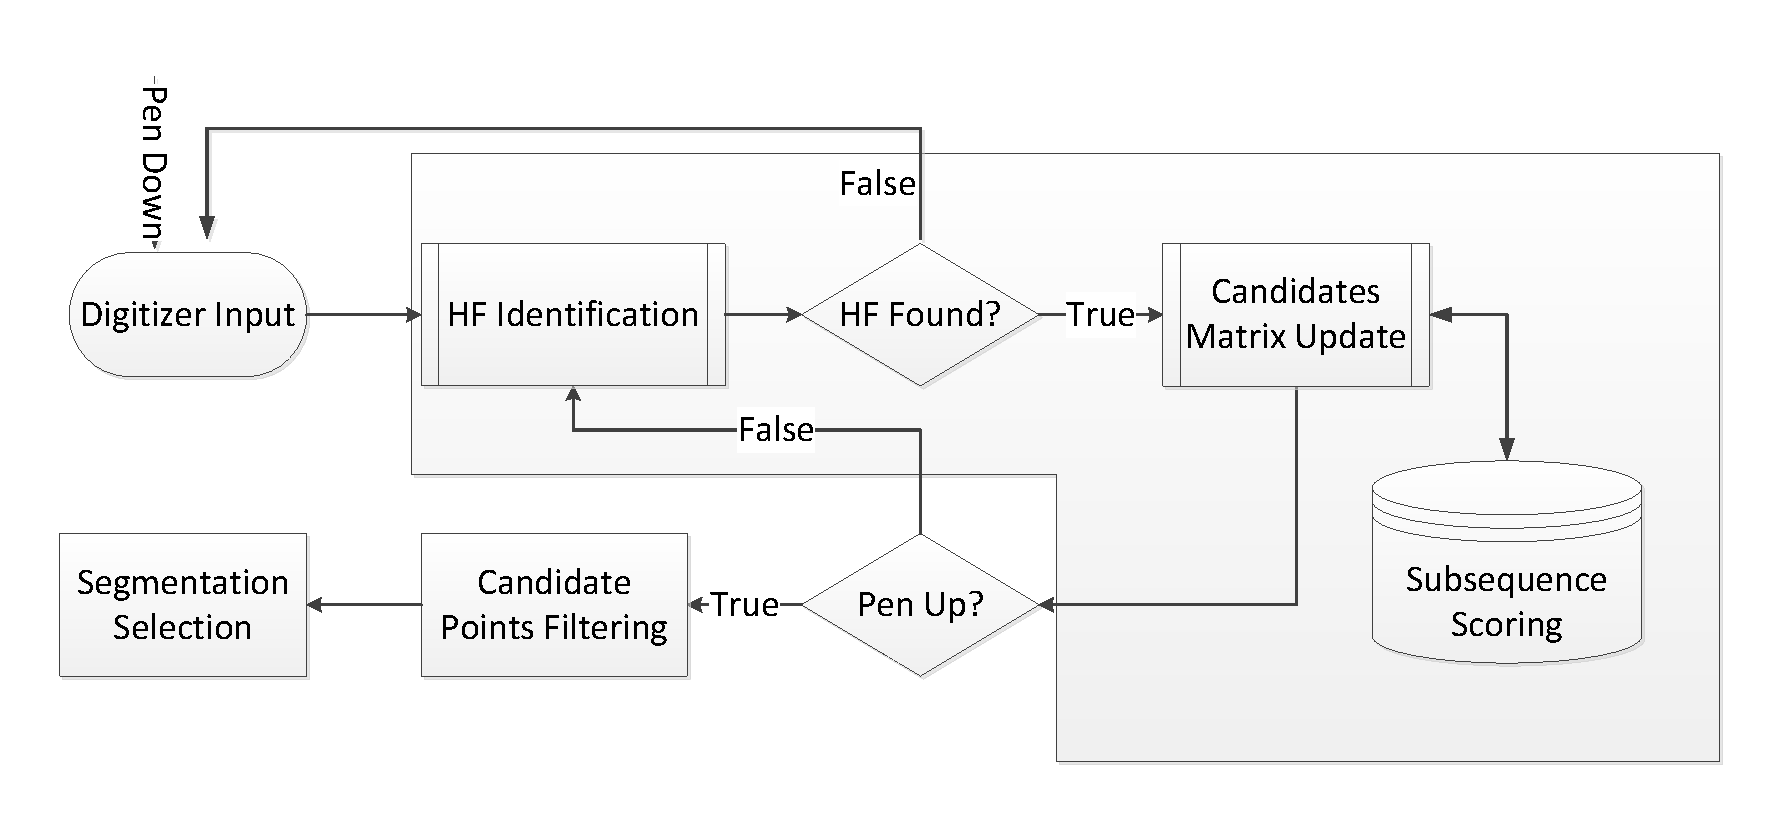
\includegraphics[width=0.9\columnwidth]{./figures/system_flow}
\caption{High level visualization of the system flow.}
\label{fig:system_flow}
\end{figure}

\subsection{First Stage: POIs Nomination and Sub-strokes Scoring}

\textbf{Horizontal fragment identification:} in this stage, the system attempts to identify \emph{horizontal fragments} (HFs) that join pairs of connected letters. 
These handlers are horizontal, directed right to left and located near the baseline (see Figure  \ref{fig:horizontal_fragments}). 
Using a smoothed version of the trajectory helps the process to ignore undesired small horizontal regions that are frequently caused by the digitizer's imperfection.  
A point $p_{i}$ is defined as a "horizontal point" if the slope of the line $\overline{p_{i-1}p_{i}}$ is less than a preset value $\delta$ which was empirically tuned to $0.6$. The same exact value for this parameter was found independently in \cite{daifallah2009recognition}.\\

\begin{figure}
\centering
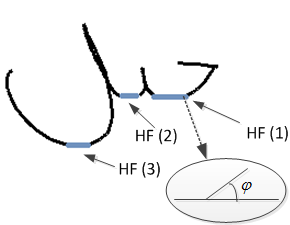
\includegraphics[width=0.5\columnwidth]{./figures/horizontal_fragments}
\caption{Horizontal Fragments [HF] of the word \RL{jbl} (JABAL).}
\label{fig:horizontal_fragments}
\end{figure}

HFs are continuously identified using the following process.
The first detected horizontal point is set as an "HF starting point". 
All the subsequent horizontal points are ignored until a non horizontal point is detected; indicating the end of an HF sequence. 
This point is identified as an "HF ending point" and the medial point of an HF is marked as \emph{point of interest} (POI). 
POI are potential SPs, thus, this process yields an over-segmentation of the stroke. 
While false positive SPs can be easily removed, missed real SPs cannot be easily recovered. 
Therefore, in order to minimize the miss-rate, this process is delicate and allows false HFs to be detected.\\

In a post processing step, fractions of the same horizontal segment, which were identified as multiple HFs, are rejoined to a single HF. 
The merging is done by evaluating the complexity measurement across the two consequent HFs, see Figure \ref{fig:candidate_in_no_horizontal}.\\

\begin{figure}
\centering
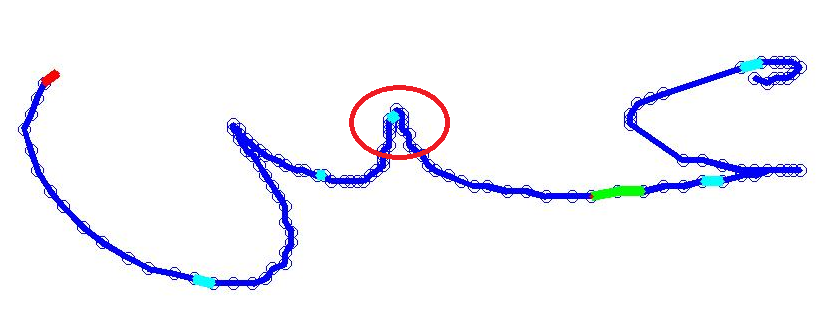
\includegraphics[width=0.5\columnwidth]{./figures/candidate_in_no_horizontal}
\caption{The main body of Arabic word \RL{`yn}. POIs are colored in cyan. The green areas indicate that the merge of HFs has taken place. Three types of false POIs can be seen: 1. A POI at the beginning of a stroke. 2. A POI that is caused by a bad HF. 3. A POI that resides in a letter valley. }
\label{fig:candidate_in_no_horizontal}
\end{figure}

\textbf{Sub-stroke Scoring:}
Let $S=\{p_{i}\}_{i=1}^{n}$ be a sequence representing a handwritten stroke in which $L$ POIs were detected. 
Let $KP=\{KP_{i}\}_{i=0}^{L+1}$ (Key Points) be the ordered set of POIs, in addition to the first and the last points of the stroke positioned as the first and the last items in the set.
Formally, we define: 
\begin{equation}
KP_{i} =\begin{cases}    1		, & \mbox{if } i=0 \\
							   POI_{i}	, & \mbox{if } 1\leq i \leq L \\
							   n    , & \mbox{if } i=L+1 
			\end{cases}				
\end{equation}

A sub-stroke $S_{i}^{j}$ is a sub-sequence of the stroke $S$ that starts at $KP_{i}$ and ends at $KP_{j}$, formally:
\begin{equation}
S_{i}^{j}=\{p_{k}\}_{k=KP_{i}}^{KP_{j}}; i<j
\end{equation}
We generate an upper triangular scoring matrix $D\in\mathbb{R}^{(L+1)\times (L+1)}$ where each cell $D_{i,j}$ represents the sub-stroke $S_i^j$. It contains the information returned by the scoring system for the sub-strokes $S_i^j$. 
The matrix $D$ is generated dynamically adding a row and a column for each new detected POI. 
Imposing a locality constraint which narrows the band of the $D$ matrix above the main diagonal improved the efficiency of the process and the segmentation accuracy. 
Given a band width $B$ we fix $D_{i,j}=\infty$ if  $j \leq i$ or $j-i>B$.
We argue that scores of sub-strokes representing a letter will achieve, in most cases, better resemblance scoring, i.e., the $D_{i,j}$ value will be relatively smaller than for other sub-strokes.\\

\begin{figure}
\centering
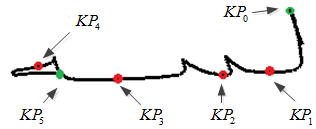
\includegraphics[width=0.5\columnwidth]{./figures/candidate_points}
\caption{Key Points of the word \RL{lbyh}. The first and last key points are colored in green. The red points are the candidate points}
\label{fig:candidate_points}
\end{figure}

The scoring system contains four databases, one for each letter position. 
It receives a sequence and a position (Ini, Mid, Fin and Iso), and returns a list of nearest neighbors samples and their scoring which indicate the similarity measure between the sequence and the candidate.
In order to reduce the number of databases which need to be accessed, we differentiate between four types of subsequences.
For each subsequence type, determined according to the location of the subsequence in the stroke, we define the letter position it may represent. 
Table \ref{table:subsequences_types} provides a mapping between the subsequence relative position in stroke and the possible letter position it may represent. In Table \ref{table:subsequences_types}, $S$ represents a stroke containing $L$ POIs where $m>0$ and $k<L+1$.\\

\begin{table}
\centering
\renewcommand{\arraystretch}{1.3}
\caption{A mapping between the subsequence types and the possible letter positions}
\begin{tabular}{| c |c | c |}
\hline
  Name     & Subsequence    & Letter Position       \\
\hline
  $\alpha$ & $S_0^{k}$         & $Ini$ or $Mid$  \\
\hline
  $\beta$  & $S_{m}^{k}$     & $Mid$              \\
\hline
  $\chi$    & $S_{m}^{L+1}$ & $Mid$ or $Fin$   \\
\hline
  $\delta$ & $S_0^{L+1}$     & All                   \\
\hline
\end{tabular}
\label{table:subsequences_types}
\end{table}

The type of the database to be examined for a given cell in $D$ is indicated in the corresponding cell in the matrix $D_p$ as in Equation \ref{eq:positions_matrix}. \\

\begin{equation}
D_{p}=
\left( 
\begin{array}{ccccccc}
\infty 	& \alpha & \alpha & \alpha  & \cdots & \alpha & \delta \\
\infty  & \infty  & \beta   & \beta   & \cdots  & \beta  & \chi    \\
\infty  & \infty  & \infty   & \beta   & \cdots  & \beta  & \chi    \\
\vdots & \vdots & \vdots  & \vdots & \ddots  & \vdots & \vdots \\
\infty  & \infty  & \infty   & \infty   & \cdots  & \beta  & \chi    \\
\infty  & \infty  & \infty   & \infty   & \cdots  & \infty  & \chi    \\
\infty  & \infty  & \infty   & \infty   & \cdots  & \infty  & \infty \end{array} \right)
\label{eq:positions_matrix}
\end{equation}
For each subsequence, the recognition system returns the $K$ minimal scored potential letters (with different labels, where the labeling is composed of the tuple (letter, position). In our case, we set $K=3$.\\


\begin{figure}
\centering
\renewcommand{\arraystretch}{1.3}
\begin{tabular}{| c |c | c | c| c | c | c |}
\hline
 $KP_i$ & $0$ & $1$ & $2$ & $3$ & $4$ & $5$\\
\hline
$0$
   & N/A
   & \subfloat{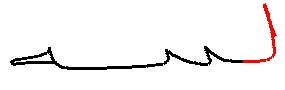
\includegraphics[width=0.8cm]{./figures/substrokes/L}}
   & \subfloat{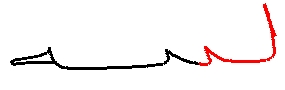
\includegraphics[width=0.8cm]{./figures/substrokes/LB1}}
   & \subfloat{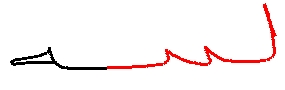
\includegraphics[width=0.8cm]{./figures/substrokes/LB1B2}}
   & N/A & N/A \\
\hline
$1$
   & N/A & N/A
   & \subfloat{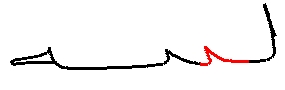
\includegraphics[width=0.8cm]{./figures/substrokes/B1}}
   & \subfloat{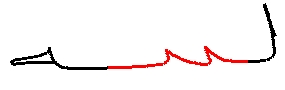
\includegraphics[width=0.8cm]{./figures/substrokes/B1B2}}
   & \subfloat{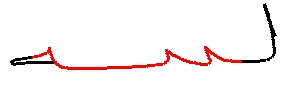
\includegraphics[width=0.8cm]{./figures/substrokes/B1B2H1}}
   & N/A \\
\hline
$2$
   & N/A  & N/A & N/A
   & \subfloat{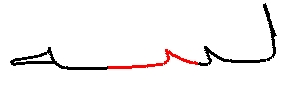
\includegraphics[width=0.8cm]{./figures/substrokes/B2}}
   & \subfloat{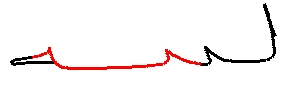
\includegraphics[width=0.8cm]{./figures/substrokes/B2H1}}
   & \subfloat{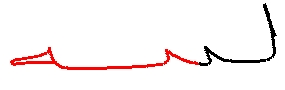
\includegraphics[width=0.8cm]{./figures/substrokes/B2H}} \\
\hline
$3$
   & N/A & N/A & N/A & N/A
   & \subfloat{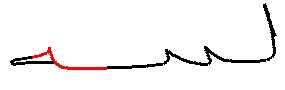
\includegraphics[width=0.8cm]{./figures/substrokes/H1}}
   & \subfloat{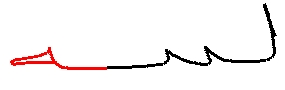
\includegraphics[width=0.8cm]{./figures/substrokes/H}} \\
\hline
$4$
   & N/A & N/A & N/A & N/A & N/A
   & \subfloat{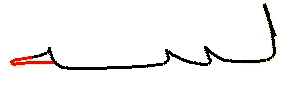
\includegraphics[width=0.8cm]{./figures/substrokes/H2}}\\
\hline
$5$
   & N/A & N/A & N/A & N/A & N/A & N/A \\
\hline
\end{tabular}
\caption{Visual demonstration of subsequences of the word shown in figure \ref{fig:candidate_points}}
\label{table:substrokes_demo}
\end{figure}

\subsection{Second Stage: Candidate points filtering and scoring correction}
In this stage we re-score subsequences and eliminate redundant POIs based on the following rules:

\begin{itemize}
	\item Inner SP (SP) lie close to the baseline. 
	\item SPs do not reside in loops.
	\item A sub-stroke length is proportional to the length of the containing stroke.\\
\end{itemize}

\textbf{Baseline detection:} The system determines the baseline by calculating the vertical density histogram of the re-sampled sub-stroke. 
The height of the stroke (y-axis) is partitioned into ten equi-length intervals. 
A POI is filtered out if it does not satisfy the following condition:
\begin{equation}
|POI_y-I_{max}| \leq 2*max{({|I|},0.15)} 
\end{equation}
where $POI_y$ represents the $y$-coordinate of the POI, $|I|$ is the length of an interval and $I_{max}$ denotes the center of the most inhabited interval. . In order to reliably determine the baseline, the algorithm is activated only after the fourth POI is detected. This process has proven to be very effective in eliminating challenging false POIs that reside in valleys of frequently used final Arabic letters, such as \RL{-q}, \RL{-s} and \RL{-n}. An example of such a POI can be seen in the letter \RL{-n} in Figure \ref{fig:candidate_in_no_horizontal}. \\

The baseline is needed only to verify that the POIs are in a reasonable distance from it, therefore, imprecise valuation of the position or the direction of the baseline is tolerable.
The third rule is used to penalize unreasonably high scoring given to small sub-strokes. 
This is done by calculating the ratio of the sub-stroke length proportional to the entire stroke length.
For instance, the suffix of the letter \RL{d} is very similar to the letter \RL{-a} and may result in a very high scoring to be granted by the recognition system. 
The only way to visually discriminate between them is by comparing the scaling of this suffix to the stroke dimensions.\\

In some cases, POIs are incorrectly nominated on non-horizontal areas. This is caused due to the fact that the nomination is done while the word is being scribed and our filtering algorithm should be corrected, in a future work, to handle this case.\\

\subsection{Third Stage: Segmentation Selection}
The goal of this phase is to select the set of SPs among the POIs. 
This set will be referred to as the \emph{Final SPs} (FSP). 
It is performed by finding the \emph{segmentation path} in $D$ with the best scoring possible. 
A segmentation path $\pi$ is an ordered subset of the KPs. 
$\pi$ must contain $KP_{0}$ and $KP_{L+1}$ as the first and the last points in the path.
$\Pi$ denotes the scoring of the segmentation path $\pi$ and defined as the summation of the scoring sub-sequences in the path. 
The lowest segmentation path determines the FSP.\\

One can model the scoring matrix $D$ as a directed, edge-weighted graph $G=(V,E)$; for which a path from vertex $KP_0$ to vertex $KP_{L+1}$ defines a possible segmentation. 
It can be experimentally validated that finding the shortest path in $G$ (from $KP_0$ to $KP_{L+1}$) does not necessarily obtain the optimal segmentation, and in some cases, produces under-segmentation of the stroke. 
It is because the shortest path is a global property which may prefer a highly weighted shortcut path over a path that consists of several low weighted fragments; in cases where the accumulative weight of the fragmented path is larger than the shortcut path.
However, greedily selecting the outgoing edge with the minimal weight will mostly return a better segmentation.\\

Several \emph{segmentation selection algorithms} (SSAs) for finding the best segmentation path are proposed in this work.
Here we describe two algorithms that were given the names \emph{Forward Segmentation Selection} (FSS) and \emph{Backward Segmentation Selection} (BSS) which operate quite similarly. 
A pseudo-code of FSS algorithm can be seen in Algorithm \ref{alg:fss}. 
FSS starts with the first point, $KP_0$, advancing toward the end of the stroke. 
In Each step, it tries to find the next best KP by selecting the adjacent subsequence $S_i^j$ with the best scoring (as can be seen in line 5). 
BSS operates similarly but starts from the last point and advances toward the beginning of the stroke. 
The main drawback of these two algorithms is that FSS tends to under-segment the suffix of the stroke and BSS tends to under-segment the stroke's prefix.\\

\begin{algorithm}
$\pi = \{1\} $\;
$i=0$\;
$sum=0$\;
\While{$i<L+1$}
{
	$j = \mathop {\arg \min }\limits_k \left( {D\left( {i,k} \right)} \right)$\;
	$\pi = \pi \cup \left\{ j \right\}$\;
	$sum = sum + D\left( {i,j} \right)$\;
	$i=j$\;
}
\caption{FSS}
\label{alg:fss}
\end{algorithm}

In an attempt to overcome the aforementioned drawbacks, a third SSA is proposed, and given the name \emph{Backward-Forward Segmentation Selection} (BFSS). 
As can be seen in Algorithm \ref{alg:bfss}, it combines both FSS and BSS. 
BFSS operates from the sides of the stroke toward the center. In every iteration, it selects two candidate points to include to the segmentation path.\\

\begin{algorithm}
$\pi = \{0,L+1\}$\;
$kp_{a}=0$\;
$kp_{b}=L+1$\;
\While{$kp_{a}<kp_{b}$}
{
	$kp_{a,next} = \mathop {\arg \min}\limits_k (D(kp_a,k))$\;
	$\pi = \pi \cup \{kp_{a,next}\}$\;
	$kp_{a}=kp_{a,next}$\;
	
	$kp_{b,next} = \mathop {\arg \min}\limits_k (D(k,kp_{b,next}))$\;
	$\pi = \pi \cup \{kp_{b,next}\}$\;	
	$kp_{b}=kp_{b,next}$\;
}

\caption{BFSS}
\label{alg:bfss}
\end{algorithm}
  
The last algorithm was given the name \emph{Greedy Segmentation Selection} (GSS) and is described in Algorithm \ref{alg:gss}.
GSS operates differently. In every iteration, the cell with the lowest (best) scoring is selected. 
Once a cell $D_{i,j}$ is selected, since it represents the sub-stroke $S_{i}^{j}$, both $KP_{i}$ and $KP_{j}$ are added to the FSP; and every cell corresponding to a subpart of the sub-stroke $S_{i}^{j}$ is removed from the scoring matrix by setting its scoring value to $\infty$; in order to avoid those sub-strokes to be selected in a later iteration.\\

\begin{algorithm}
$\pi = \{0,L+1\}$\;
\While{$D \neq [\infty]^{(L+1)\times (L+1)}$}
{
	${s,e} = \mathop {\arg \min}(D)$\;
	$\pi = \pi \cup \{s,e\}$\;
	$sum = sum + D(s,e)$\;
	$UpdateMatrix(D,s,e)$\;
}

\caption{GSS}
\label{alg:gss}
\end{algorithm}

FSS, BSS, BFSS and GSS are executed independently; each returning a segmentation path. The segmentation path with the smallest $\Pi$ is selected and the $FSP$ is determined. Performance evaluation of the mentioned SSA is provided in \ref{subsec:ssa_performance}. \\

\section{The ADAB Database}
\label{sec:database}
The ADAB database is, de-facto, a standard in the field of on-line Arabic handwriting recognition. It is freely available and consists of more than 20k Arabic handwritten words (937 
Tunisian town/village names) scribed by more than 170 different writers. 
Unfortunately, the ADAB only provides data on the strokes for a given city name. 
No segmentation into letters or \emph{word parts} (WPs) is provided by the database; thus, extra work was needed to add this information in order to use its letter samples and as a ground truth for the segmentation system.
To provide this information, we employed the skills of a human expert to segment the strokes into letters, and to determine the words and the WP boundaries for each sample. 
This additional information was saved in an XML file. Delayed strokes were not included in the processed information since it is not considered by the segmentation process.
We have manually segmented more than 15k samples that contain about 40k strokes. \\

\begin{figure}
\centering
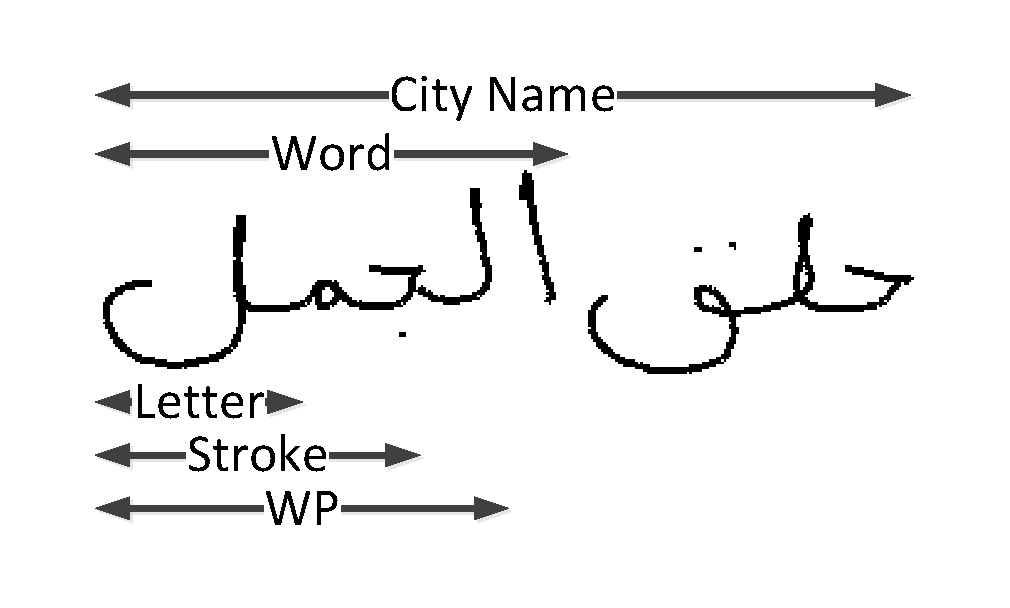
\includegraphics[width=0.6\columnwidth]{./figures/sample_parts}
\caption{The parts of a sample in the ADAB database.}
\label{fig:sample_parts}
\end{figure}

\section{Validation}
\label{sec:validation}
Related researches usually use a human expert to validate the accuracy of the SPs. However, in this work, we applied an automatic validation process using the ground truth information provided by the database. We discriminate between three types of final SPs. A final SP is classified as true positive if the complexity measure between the identified point and a true SP is less than a preset threshold; otherwise it is classified as false positive. A false negative (miss), is the case when the system failed to identify a true SP. The validation process was tested on several sets and found to be highly reliable.\\

\begin{figure}
\centering
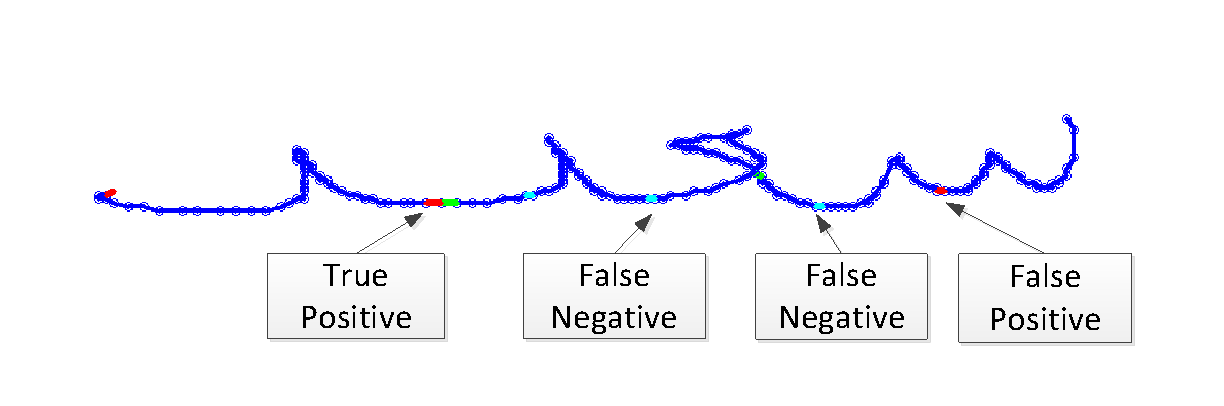
\includegraphics[width=0.8\columnwidth]{./figures/sp_types}
\caption{SPs types.}
\label{fig:sp_types}
\end{figure}

\section{Experimental Results}
\label{sec:results}
The system was implemented using Matlab environment. Comparing the performance of the proposed approach to results obtained by in related researches could be difficult due to the different experimental settings, databases and methodology; not to mention the different measures that are used in presenting the results. The usage of the ADAB database, instead of a self-collected database, standardize and reinforces our results. In Table \ref{table:general_stats} we provide basic statistics of our sample set.

\begin{table}[h]
\caption{General statistics}
\renewcommand{\arraystretch}{1.2}
\begin{tabular}{ | c | c | }
  \hline
  Number of test samples (city name) & 319 \\
  \hline
  Number of WPs & 1148 \\
  \hline
  Number of Strokes & 1237 \\
  \hline
\end{tabular}
\centering
\label{table:general_stats} 
\end{table}

The results shown in Table \ref{table:results} summarizes the system's performance. The absolute majority of the false negative SPs were identified as POIs in the first stage. A small number were filtered out in the filtering phase but most of them were not selected by the SSA.\\

\begin{table}[h]
\caption{Results}
\renewcommand{\arraystretch}{1.2}
\begin{tabular}{ | c | c | }
  \hline
  Strokes segmentation rate (SR) &  83\% \\ 
  \hline
  Strokes recognition rate (RR) &  78\% \\ 
 \hline
  Total number of true SPs & 1081 \\
  \hline
  Valid SPs (True Positive) & 85.3\% \\
    \hline
  Missing SPs (False Negative) & 14.7\% \\
  \hline
  Invalid SPs (False Positive) & 119 (11\%) \\
  \hline                                    
  SPs Precision & 88.6\% \\ 
 \hline
  SPs Recall &  85.3\% \\ 
 \hline
\end{tabular}
\centering
\label{table:results} 
\end{table}

\subsection{Analysis}
In this section we discuss common cases of incorrect segmentation.
\subsubsection{Over-segmentation}
\begin{itemize}
\item Several Arabic letters contain a horizontal region in their initial form which does not accommodate a SP. We overcame this problem by adding the following rule: A POI is nominated only if the sub-stroke that spans from the beginning of the stroke to the POI has a high complexity measure.
\item Over-segmentation can also be caused by typing a letter in unusual form where it is spanned over several strokes. 
It happens mostly in the letter \RL{-m-}, \RL{-m} and in rare cases in the letter \RL{-.h-}. This issue will be addressed in a future work.
\end{itemize}

\subsubsection{Under-segmentation}
\begin{itemize}
\item Letter pairs that are not separated by HFs cause the system to miss POIs. This issue was partially solved by extending the notion of a letter to include such pairs. For example the pair \RL{lm} and \RL{l.h}.
\item In some cases, HFs were identified correctly but the corresponding POI were not selected in the third stage. \\
\end{itemize}

In addition, differentiating between the main body of the letter \RL{-s-} and the main body of two consecutive \RL{-b-} letters is possible only when considering additional strokes, thus both cases were considered to be correct.\\

\subsection{Segmentation Selection Algorithms Performance}
\label{subsec:ssa_performance}
As can be seen in Table \ref{table:ss_algorithms_results} the SSA has a crucial effect on the system's performance. We tried different combinations of two SSAs. The selection of the FSP is done by running both SSAs and selecting the segmentation path with the smallest scoring divided by the number of SPs. This is done in order to prevent giving superiority to FSPs with less SPs. In Table \ref{table:ss_algorithms_results}, a combination of two algorithms is denoted by $\oplus$.\\

\begin{table}[h]
\caption{SSAs Performance}
\renewcommand{\arraystretch}{1.2}
\begin{tabular}{ | c | c | c | c | c |}
\hline
SSA & WP SR & WP RR & SP Precision & SP Recall\\
\hline                 
  FSS & 76\% & 70\% & 85\% & 78\% \\ 
  \hline
  BSS & 79\% &  73\% & 84\%& 81\% \\
  \hline
  BFSS & 78\% & 72\% & 84\% & 80\%\\ 
  \hline
  GSS & 80\% & 74\% & 81\% & \bf{94}\% \\  
  \hline
  FSS$\oplus$BSS & \bf{82}\% & \bf{76}\% & \bf{89}\% & 82\%\\  
  \hline
  GSS$\oplus$BFSS & 81\% & 75\% & 83\% & 90\% \\
  \hline
\end{tabular}
\centering
\label{table:ss_algorithms_results} 
\end{table}

\subsection{Sample set size and distribution}
Since our samples are extracted from a database with a limited dictionary diversity, the letters sample set distribution is imbalanced. 
On one hand, it can be considered an advantage since the sample set distribution reflects the a-priory probability of a letter appearance test set. 
On the other hand, a highly imbalanced dataset is known to negatively affect many classification algorithms.
In the following experiment, we measure the affect of an increasingly large and imbalanced training set on the system's performance increasing the maximal number of samples per letter position allowed to be included in the sample set and then measure the WP segmentation and recognition rates. 
Note that increasing the maximal number of samples per class (letter position) increases the imbalance between the classes. 
The graph in Figure \ref{fig:num_letter_impact} shows that the system performance convergences when the maximal number of samples is larger than 200 per class (letter and position). 
It is also evident that there is a point where allowing more samples per class may decrease the accuracy of the system;
and that the recognition rate (RR) is more sensitive to the sample size than the segmentation rate (RR). \\

\begin{figure}
\centering
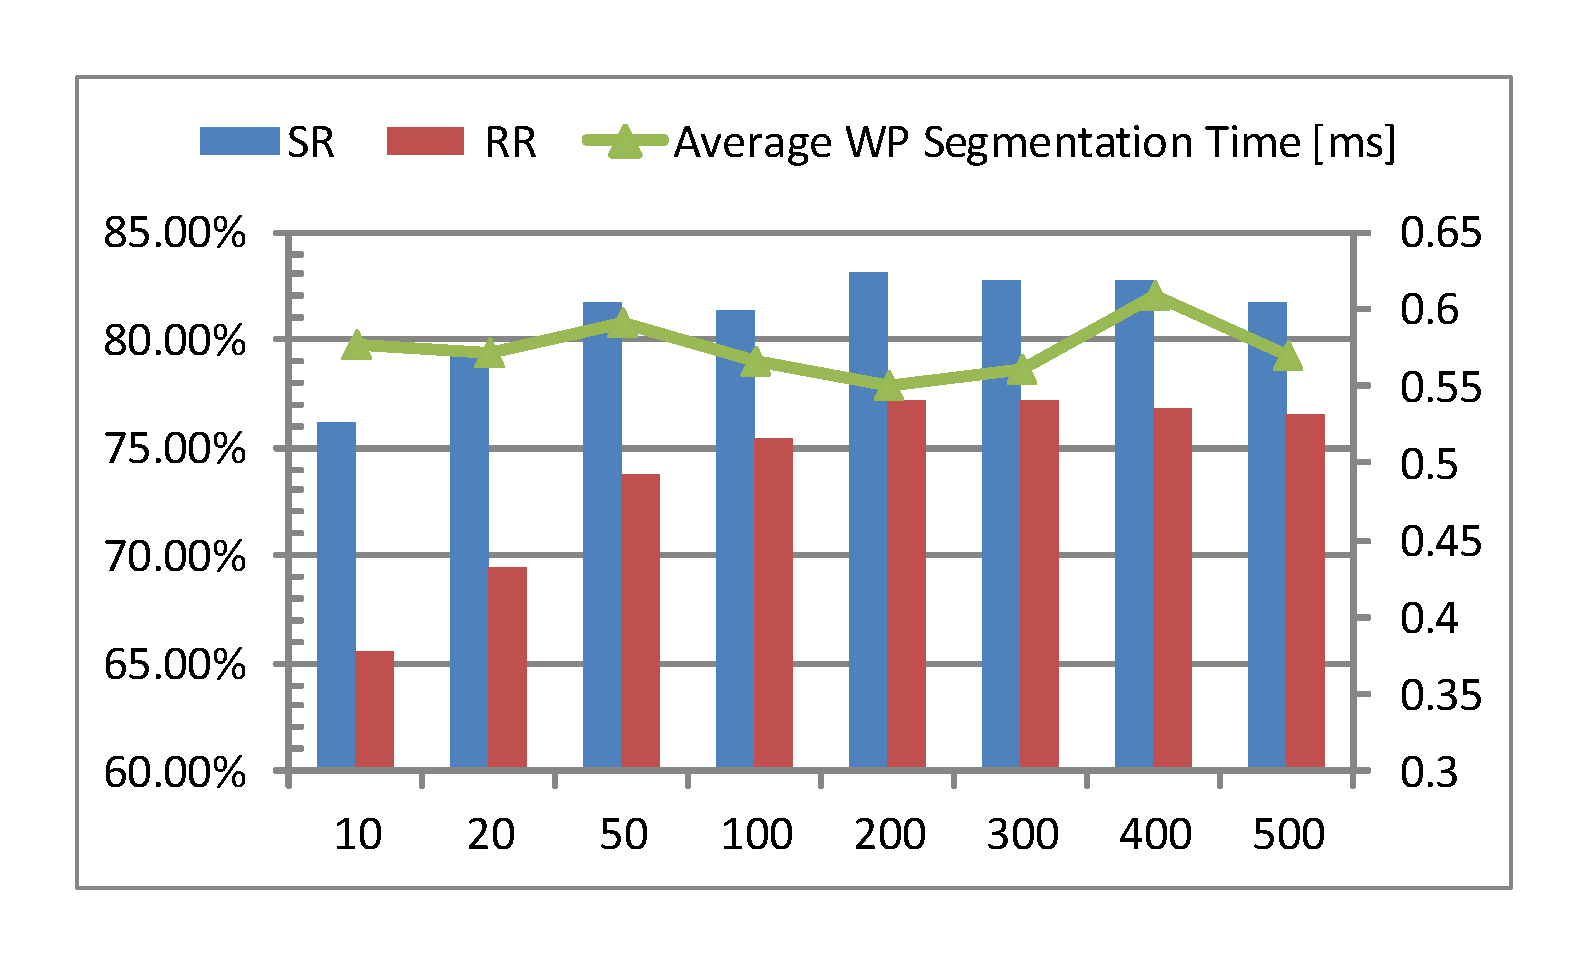
\includegraphics[width=0.9\columnwidth]{./figures/num_letter_impact}
\caption{The diagram shows the impact of the increase of maximal number of samples per class on the segmentation and recognition rates.}
\label{fig:num_letter_impact}
\end{figure}

\section{Conclusions and Future Work}
In this paper we proposed an ongoing approach for segmenting dictionary-free Arabic handwritten script in the stroke level, based on continuous sub-strokes scoring. The nomination of potential SPs is done based on morphological features and a letter recognition system is used to provide scored letter candidates to the sub-strokes that are induced by the nominated points. The  system has demonstrated promising results.
In future work, we will extend the process by adding a holistic recognizer that uses the segmentation and the scoring information to limit the number of potential dictionary words to be inspected.\\

\section{Acknowledgment}
We would like to thank Professor Dana Ron, from the Tel-Aviv University, for her invaluable help in this research and her insightful comments on this paper. \\

\bibliographystyle{IEEEtran}
\bibliography{IEEEabrv,bibliography}

\end{document}


